%*******************************************************************************
%*********************************** First Chapter *****************************
%*******************************************************************************

\chapter{Introduction}  %Title of the First Chapter 

\graphicspath{{Chapter1/Figures/} {Chapter1/Figures}}
\begin{quote}
\textsl{One should never try to prove anything that is not almost obvious - Alexander Grothendieck}
\end{quote}


\section{Introduction}

We live in a world where information is being bombarded on our cognitive faculties from all sides, at all times. The internet is a continuous stream of information and each source is fighting with the other to get a piece of our attention budget. 
With the advent of machine learning and big-data sources, building systems that predict actions as a response to perceptual triggers is the bread and butter of many companies. The use cases may range from understanding which advertise made a visitor do an unscheduled purchases on amazon, or which string of music tracks recommendations maximized a users time on a particular music platform. But in the end it all boils down to understanding what triggers result in human action or lack there of\cite{song2012survey}. Nonetheless the systems that surrounds a human interacting with the internet, are all figuring out the best triggers which are perceived by the human as worthy of attention. 
The term ``Attention Economy''\cite{davenport2001attention} was actually coined for this very reason. In the words of Matthew Crawford ``\textit{Attention is a resource, a person has only so much of it.}''\cite{MatthewCrawford}. We live in the age of distraction, and more often than not, our perceptions are guiding our actions, than our cognitive processes. Several studies have shown that engagement is almost always a game of stimulating our most basic urges, such as dopamine hits, presence of faces or simply arousal of emotions to increase the working memory.\cite{bakhshi2014faces,joglekar2017like}\cite{schupp2006emotion}\cite{soat2015social}. 
An interesting side effect of dwindling attention budgets is the emergence of more formal topical spaces on the internet. The ever pervasive nature of the internet allow these formal spaces to function almost like physical communities, with moderated and effective peer to peer exchange of thoughts, ideas and empathy\cite{kummervold2002social,squire2015should,hwang2010social}.

In such an environment, as computer scientists, it is worth asking the question: \textbf{Can we develop pipelines that can look at the structures in the data to quantify how humans perceive their sphere of interaction? Can we use that perception to design impactful interventions towards well being of the users, on and off the internet?}. 
This question can be decoupled and decomposed into two fundamental problems:
\begin{enumerate}
\item How do human perceptions manifest in data? 
\item How do we quantify these perceptions?
\end{enumerate}
These two questions are going to be the guiding principles of my dissertation. 

But first of all, we need to clarify the relation between perception, affects and intervention and to do so we should try and understand each of these terms separately as a part of the native field's context.

\section{Perception and Affect}
\note{This paragraph needs to be refined with more literature that convinces the reader that perception -> emotion. And any knowledge extraction pipeline inherently links the two together.}
In this dissertation, I would try to build frameworks to capture human perceptions in the realm of human to human interactions and subjective aesthetics. The utility of such an attempt, can only be justified if there is a real link between how humans function at the most fundamental cognitive level and how they perceive the intangible, including the aesthetic. There has been an ongoing effort to unravel this link, through psychological, neuro-evolutional and philosophical arguments. I will try to gain inspiration from them, but a detailed critique is beyond the scope of my dissertation and expertise.
\textsl{\textbf{Affect (APA definition):} any experience of feeling or emotion, ranging from suffering to elation, from the simplest to the most complex sensations of feeling, and from the most normal to the most pathological emotional reactions.}\\
\textsl{\textbf{Perception (APA definition):} the process or result of becoming aware of objects, relationships, and events by means of the senses, which includes such activities as recognizing, observing, and discriminating. These activities enable organisms to organize and interpret the stimuli received into meaningful knowledge and to act in a coordinated manner.}\\

Emotions or `affects' and perceptions have long been discussed in the psychology, neuroscience and philosophical literature. Emanuel Kant in his prolific work, first discussed the utility and the philosophical reasoning behind presence of affects or emotions\cite{kant1987critique}. In his opinion, emotions are pre-cognitive involuntary states, termed as "mere perceptions of unspecified bodily states"\cite{borges2004can}. But that does not mean they don't influence our deepest level of well-being.
The link between affect and perception has also been explored in several cases. An argument to link perception of affect arousing aesthetics was made by Perlovsky\cite{perlovsky2014aesthetic}, where they propose that the phenomenon of affects arousing from aesthetics, comes from a fundamental human need enrich the knowledge bases about real world. An unexpected thing of structure, satisfies this need at some level and we perceive it as aesthetically pleasing. Another recent study by Zadra et.al\cite{zadra2011emotion} evaluated the relation between visual perception and emotions. They demonstrate that the conventional assumption of the disentangled functioning of perception and affects is not necessarily true. Humans are quite susceptible to perceiving different realities based on different aroused affects. 

So the community is still unclear, but there seems to be a theory that  

\section{Intervention and the DIKW model}

\begin{figure*}[t!]
    \centering
    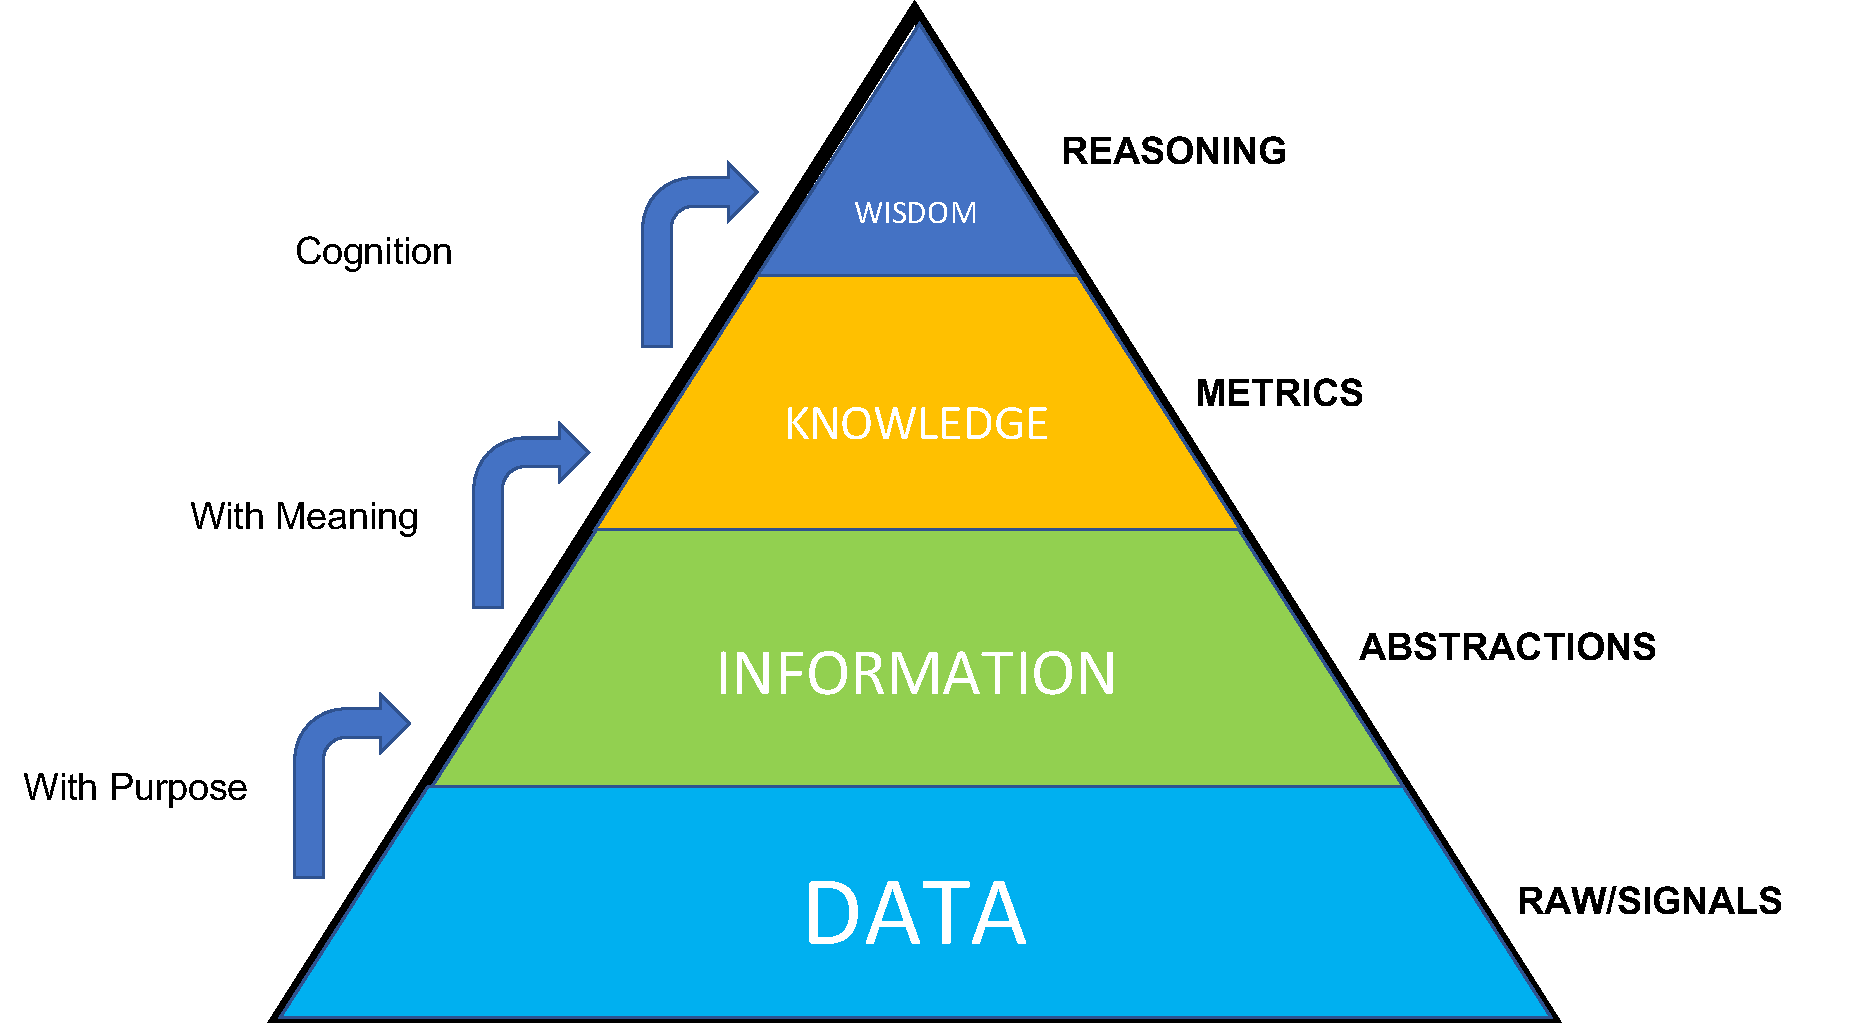
\includegraphics[width=\columnwidth]{DIKW.pdf}
    \caption{The DIKW pyramid}
    \label{fig:dikw}
\end{figure*}


The reflection to find the answers the questions, ties us back to one of the fundamental frameworks about operations on data, that is the \textbf{Data , Information, Knowledge and Wisdom} model\cite{rowley2007wisdom}.In this dissertation I posit and demonstrate through case studies, that for reasoning about perceptions, you need to interpret the metrics that contain contextual knowledge about the abstractions you are working with through the lens of the target ontology. Debating the nature of this ontology is not the purpose of this dissertation, but I show that `a' solution can be reached, if systems are designed to interpret metrics by anchoring around an ontological bias.

In this model, the most base layer consists of the pure form raw \textbf{data or signals} that come from a source. If we are measuring perceptions of human, this source needs to be tied back to humans in some way. The data needs to be generated as a result of some human-human interaction or as a result of deliberate human input as a form of response to their perception of some event. 

The \textbf{information} layer is the result of the fact that any process done on the data is with a sense of purpose or an end goal. For example, if the goal is to understand how humans exchange messages at times of distress, you would most certainly need to express the raw information about sender and recipient of messages into some form of a networked abstraction. The abstraction preserves the organization of data, but at the same time allows information to be operated on. As a result, almost always the output of this process is some form of a data abstraction. In the next stage of processing, you need to attach some meaning to the patterns in the information to extract 

\textbf{knowledge}. This  For example, if you need to know the most popular user who has exchanged the most messages with others among a network of users exchanging messages; you would look for the most central user in the network. In this particular case, the metric of centrality dawns the meaning of popularism in the context of our message network. 

The final layer needs a cognitive process and an ontological framework, to extract actionable insights, which we can call \textbf{wisdom}, from the knowledge. By classical definition of ontology, it defines properties of and relations between objects. For this very reason, these ontological frameworks need to be originating from the field of intervention.  In our example, a human analysing data needs to get some insights about the dynamics of popular users which requires the human to consume the metrics and derive insights. However the insights need to be grounded in psychological ontological framework, for us to derive certain trends in behavioural dynamics of this network.  Figure \ref{fig:dikw} shows an illustration of the adopted version of Rowley's DIKM model. 

\subsection{Data}
As discussed, this dissertation is about developing frameworks around quantification of human perceptions, such that we can do impactful interventions from this approach. And the most base level of this pyramid is the data that the frameworks would work with in order to progress on these lines. I work with two forms of data, textual data and image data, to understand two separate forms of perceptions. 

\subsubsection{Textual Data}
The first case study of this dissertation focusses on is online support communities. It has been shown through several studies in medical informatics, that these communities play a very important role in providing support and respite in times of distress. The communities are especially helpful when it comes to people suffering from long term illnesses or mental health issues. 
To understand how users on these communities perceive social support, I work with data acquired from online health forums, where users share, give support and ask for support. I look at communities that deal with long term conditions like Lung illnesses, and communities where mental health patients seek support. 

\subsubsection{Image data}
The other facet of my work looks for quantification of how we perceive physical spaces. I work with google street view data, and the aim of this work is to understand, through crowd sourced methods, how people perceive the sense of beauty in urban areas. 

\subsection{Abstractions}
As mentioned before, the act of aggregating information from data, almost always involves building organized abstractions. In case of the first study with textual data, I incorporate user information into the textual data to build organized networked structures, which can then be evaluated using graph theoretic methods. To understand textual patters, I use the language embedding models which would be discussed in the chapters to come. 
While processing image data, I use several segmentation techniques to group semantically similar pixels together. I also use several state of the art object and scene detection to extract semantic information from an image. A more detailed discussion of these abstractions would be done in the later chapters.  

\subsection{Knowledge}
For extracting knowledge, we need to first associate meanings to certain computable metrics that we obtain from the abstractions. As discussed in the previous example, it could be as simple as associating the property of ``popularity'' to the metric of centrality. In my case, I develop several of these metrics for the two studies, some based on intuitions which i test validity for, and some based on extensive literature survey. To give an example, I develop the concept of anchored triads, which combines local interaction motifs with the role of a user in a supportive conversation to understand how these conversations evolve. 

\subsection{Wisdom}
Finally the wisdom in my case, is simply the philosophical, quantitative and qualitative discussion about what perception did we actually capture from these progressive operations. To answer the questions posed by this layer, we need to hold on to \textbf{an ontological framework} which grounds the metrics in the field of human interaction and planned intervention. This ontological framework that deems meaning to the structure in data, needs to be achieved through cross disciplinary literature review. In case of social support, what metrics combined with the understanding of human behavioural ontology, give rise to signatures of social support? Could those be found in sociological literature that distils social ties as interaction motifs? Or can that be found in pure statistical understanding of networks and formation of edges?  And in the end, can we provide valuable interventions in the scenarios where humans are asking for help online. My dissertation navigates similar questions to arrive at 'an approach' to quantify and intervene using signatures of human perceptions from data.

\section{Research hypothesis}
The global hypothesis of my dissertation as described before comprises of asking the two aforementioned questions: \textbf{How do human perceptions manifest in data?} and \textbf{How do we quantify these perceptions?}. But these questions are quite open ended, and answering them in a generalized manner seems impractical. For this reason, I need to first contextualize my work in the realm  of practical applications. 
To rationalize the pursuit of these questions, I choose application driven case studies, which allow me the luxury to do a data driven exploration with a final goal of designing intervenable frameworks.
Across my investigations, I follow the DIKW framework layer by layer, by distilling actionable wisdom from data. Through the two case studies , my work touches a diverse set of data science tools  which range from complex networks formulations to generative adversarial models of human perception.

My research explores the following global hypotheses using the two case studies. 

\subsubsection{H1: Data about human interactions from the web can be used to capture signatures of perceptual processes  } 


\subsubsection{H2: Human interactions data from the web can be used to quantify subjective attributes of the real world}

\subsubsection{H3: These quantifications can be effectively used to drive intervenable insights to improve perceptions of the said humans. }



Human interactions data from the web can be used to capture peculiar formats of human conversations



Ontology in a philosophical context is a branch of metaphysics, which asks the questions like "What exists?", "What comprises an object? ", "What hierarchies of object classes are present?", "What different entities form a higher entity?". Naturally this framework was suitable in information sciences to describe datum as hierarchies or taxonomies of other objects. 



\section{Thesis overview}

In the first study, I examine the structure behind how people seek engagement on-line. I discover that humans are very limited by their attention budgets, and engage with informal social networks in a very atomic and primacy driven way, which makes prediction of engagement using certain attributes of the content very feasible. But on the contrary, in more formal social networks, where the aim is to exchange knowledge and support, the network evolves around certain key elements of perception of support and helpfulness, which are well explored in the real world communities. On the journey to unravel these traits, I develop techniques to abstract out online formal conversations and develop a models for detecting supportive conversations on the web. I discuss the utility of such a model and draw parallels with the offline model of community support. 

In the second study, I investigate utility of perceptions of real world places through a crowd sourced rating of google street view images. I develop models to extract the perception of the crowds using data driven inference methods.
I show that a general pattern of beauty in urban spaces can be learnt through a crowd sourced opinion and based on this finding, I develop a generative model to simulate beautification of urban spaces by using deep learning. I validate the quantification of perception of real-world beauty using crowd validation. I contribute a way to use computer vision techniques to abstract out beautification process into explainable metrics used by architects and urban planners. The final contribution is a demo web application, that allows practitioners to examine and validate the utility of such a end to end system that captures citizen perceptions for urban design. 




\section{Original contributions}


\section{Outlook}




\subsection{Notes}

Some points to cover in introductions 

\begin{itemize}
    \item Kant's theory of emotions , and how stimulus -> cognition -> emotion and  action links everything together 
    \item importance of capturing affects (desire to influence behaviour)
    \item There have been attempts to capture this , and how the plutchik's frameworks has helped in distilling certain emotions and capturing them from different forms of media 
    \item this dissertation takes an different approach, in which we try to find signatures of affective responses seen online 
    \item the dissertaion works in two parts, the first part looks at how support can be detected from structures in coversation 
    \item part 2 looks at how the affect of beauty impacts how citizens perceive cities and can we capture that affect to improve urban design process  
\end{itemize}








